\documentclass{article}

\usepackage{siunitx} % Provides the \SI{}{} and \si{} command for typesetting SI units
\usepackage{graphicx} % Required for the inclusion of images
\usepackage{amsmath} % Required for some math elements 
\usepackage[export]{adjustbox} % loads also graphicx
\usepackage{listings}
\usepackage{matlab-prettifier}
\usepackage{float}
\usepackage[most]{tcolorbox}
\usepackage{amsfonts}
\usepackage{color}
\usepackage{titlesec}
\usepackage{caption}
\usepackage{subcaption}

\newcommand{\R}{\mathbb{R}}

\usepackage{xcolor}

\DeclareCaptionFont{white}{\color{white}}
\DeclareCaptionFormat{listing}{%
  \parbox{\textwidth}{\colorbox{gray}{\parbox{\textwidth}{#1#2#3}}\vskip-4pt}}
\captionsetup[lstlisting]{format=listing,labelfont=white,textfont=white}
\lstset{frame=lrb,xleftmargin=\fboxsep,xrightmargin=-\fboxsep}
\titleformat{\section}[runin]
  {\normalfont\Large\bfseries}{\thesection}{1em}{}
\titleformat{\subsection}[runin]
  {\normalfont\large\bfseries}{\thesubsection}{1em}{}


\setlength\parindent{0pt} % Removes all indentation from paragraphs

\renewcommand{\labelenumi}{\alph{enumi}.} % Make numbering in the enumerate environment by letter rather than number (e.g. section 6)

%\usepackage{times} % Uncomment to use the Times New Roman font

%----------------------------------------------------------------------------------------
%	DOCUMENT INFORMATION
%----------------------------------------------------------------------------------------

\title{AMATH 353: Homework 12 \\Due May, 18 2018 \\ ID: 1064712} % Title

\author{Trent \textsc{Yarosevich}} % Author name

\date{\today} % Date for the report

\begin{document}
\maketitle % Insert the title, author and date
\setlength\parindent{1cm}

\begin{center}
\begin{tabular}{l r}
%Date Performed: December 1, 2017 \\ % Date the experiment was performed
Instructor: Jeremy Upsal % Instructor/supervisor
\end{tabular}
\end{center}

% If you wish to include an abstract, uncomment the lines below
% \begin{abstract}
% Abstract text
% \end{abstract}

%----------------------------------------------------------------------------------------
%	SECTION 1
%----------------------------------------------------------------------------------------
\section*{Part 1}
Assuming $u(x, t) = u(x(t), t)$ , by the chain rule we have $\frac{d}{dt}u = u_t + u_x\frac{dx}{dt}$. Given that we are solving $u_t + 2u_x = 0$, if we assume $\frac{dx}{dt} = 2$ we get the following:
\begin{equation}
\frac{d}{dt}(u(x(t), t)) = u_t + 2u_x = 0
\end{equation}
This gives us the two ODEs:
\begin{tcolorbox}[minipage,colback=white,arc=0pt,outer arc=0pt]
\begin{equation}
\begin{aligned}
\frac{dx}{dt} = 2\\
\frac{du}{dt} = 0
\end{aligned}
\end{equation}
\end{tcolorbox}
Solving the first ODE by separation of variables, we get the following equation for the characteristic curves, which are shown in the plot below:
\begin{equation}
x(t) = 2t + x_0
\end{equation}
\begin{figure}[H]
  \centering
    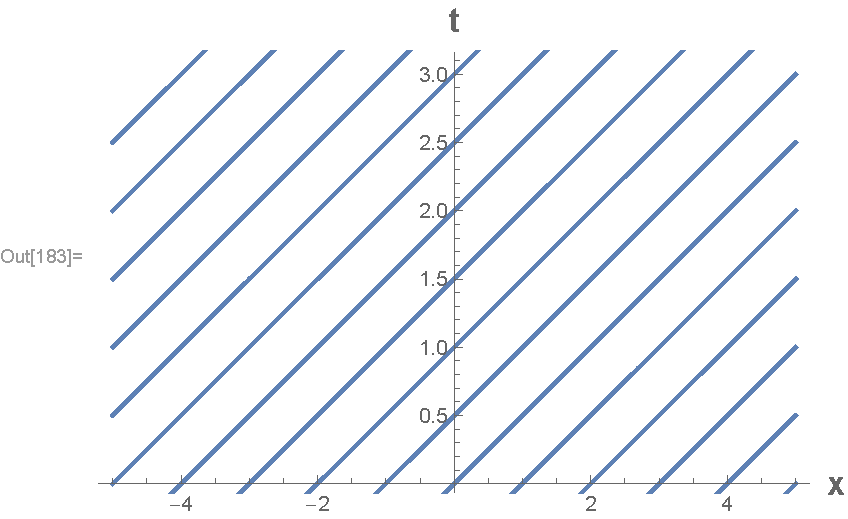
\includegraphics[width=\textwidth]{hw_12_plot1.pdf}
    \caption{$t = \frac{x-x_0}{2}$}
\end{figure}
Solving the second ODE we simply get a constant:
\begin{equation}
\begin{aligned}
\int \frac{du}{dt} = \int 0dt\\
u(x(t), t) = A
\end{aligned}
\end{equation}
Making use of the initial condition, $u(x, 0) = e^{-x^2}$ we have the following:
\begin{equation}
\begin{aligned}
u(x(t), 0) = u(x_0, 0) = u_0(x_0) = A\\
u_0(x_0) = e^{-x_0^2}\\
A = e^{-x_0^2}\\
\end{aligned}
\end{equation}
\begin{tcolorbox}[minipage,colback=white,arc=0pt,outer arc=0pt]
\begin{equation}
u(x(t), t) = e^{-x_0^2}
\end{equation}
\end{tcolorbox}
This means that along any given characteristic line $u(x, t) = u(x(t), t)$ we have $u$ constant at a value determined by the initial value of that particular characteristic.\\
\\
Now using an example of a point $(3,4)$ we plug it into the characteristic curve and determine it's $x_0$ value, then determine the value of $u_0$ at that point, and thus $u$ along that entire characteristic curve:
\begin{equation}
\begin{aligned}
x_0 = x - 2t\\
x_0 = 3 - 4(4) = -5\\
\end{aligned}
\end{equation}
\begin{tcolorbox}[minipage,colback=white,arc=0pt,outer arc=0pt]
\begin{equation}
u_0(-5) = e^{-(-5)^2} = e^{-25}
\end{equation}
\end{tcolorbox}
We can arrive at the same value generally by plugging the $x_0$ equation into the equation derived above for $u(x(t), t)$, then plugging $(3,4)$ into that:
\begin{equation}
\begin{aligned}
x_0 = x - 2t\\
u(x(t), t) = e^{-x_0^2}\\
u(x, t) = e^{-(x - 2t)^2}\\
\end{aligned}
\end{equation}
\begin{tcolorbox}[minipage,colback=white,arc=0pt,outer arc=0pt]
\begin{equation}
e^{-(3 - 2(4)^2} = e^{-25}
\end{equation}
\end{tcolorbox}
Note the results of (8) and (10) are the same.
\section*{Part 2}
\subsection*{a.)}
The characteristic curves and ODEs for this question are arrived at in the same manner as equations (1) - (4) above, albeit restricted to $x \geq 0$:
\begin{tcolorbox}[minipage,colback=white,arc=0pt,outer arc=0pt]
\begin{equation}
\begin{aligned}
\frac{dx}{dt} = 2\\
x(t) = 2t + x_0\\
\frac{du}{dt} = 0\\
u(x(t), t) = A
\end{aligned}
\end{equation}
\end{tcolorbox}
Note that $x_0 = x - 2t$, and so with the restriction that $x > 2t$, we can assume that $x_0$ will be positive, and thus will be defined by the initial value $u(x, 0) = 0$. We can then use this to solve the constant in $u(x(t), t)$:
\begin{equation}
\begin{aligned}
u(x(t), t) = A\\
u(x(t), 0) = u_0(x_0) = A\\
u_0(x_0) = 0\\
A = 0
\end{aligned}
\end{equation}
From this it follows that when $x > 2t$:
\begin{tcolorbox}[minipage,colback=white,arc=0pt,outer arc=0pt]
\begin{equation}
u(x, t) = 0
\end{equation}
\end{tcolorbox}
\subsection*{b.)}
To solve for $u$ when $x < 2t$, I took the same approach, but integrated $\frac{dx}{dt}$ differently in order to get $t$ in terms of $x$ and some $t_0$:
\begin{equation}
\begin{aligned}
\frac{dx}{dt} = 2\\
dt = \frac{2}{dx}\\
\int dt = \int \frac{2}{dx}\\
t = \frac{1}{2}x + t_0
\end{aligned}
\end{equation}
From this equation we can see that $t_0 = t - \frac{1}{2}x$ and so when $x < 2t$, the value of $t_0$ will be greater than $0$ and thus defined by the initial condition $u_0 = u(0,t) = \frac{t}{1+t^2}$. From this, we follow the same procedure as above to solve for $u$:
\begin{equation}
\begin{aligned}
u(x(t), t) = A\\
u(0, t) = u_0(t_0)\\
u_0(t_0) = \frac{t_0}{1+t_0^2} = A
\end{aligned}
\end{equation}
Then plugging in the value above for $t_0$ we arrive at the solution for the value of $u(x, t)$ when $x < 2t$:
\begin{tcolorbox}[minipage,colback=white,arc=0pt,outer arc=0pt]
\begin{equation}
u(x, t) =  \frac{t - \frac{1}{2}x}{1+(t - \frac{1}{2}x)^2}
\end{equation}
\end{tcolorbox}
Here are the profiles of the solution at $t = 0, 1, 2, 3$ (note that at $t=0$ the solution is of course 0 for all $x$).
\begin{figure}[H]
  \centering
    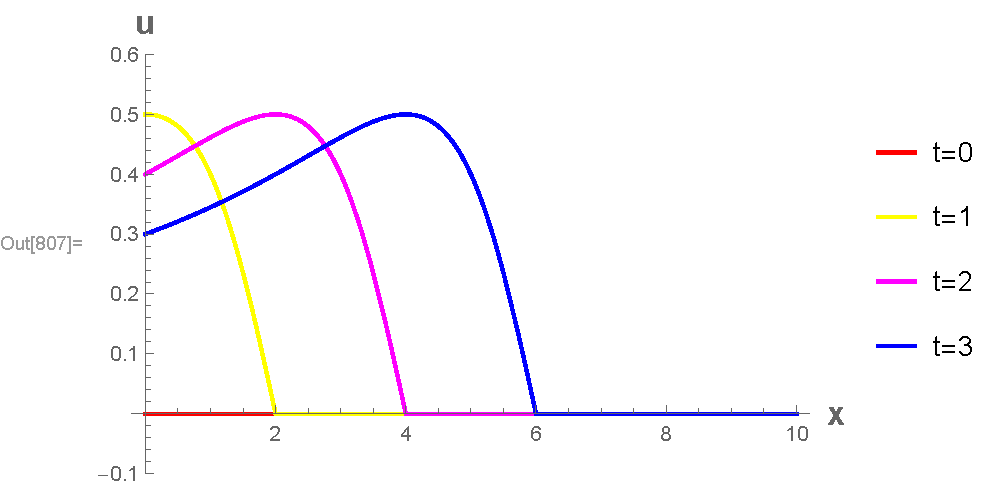
\includegraphics[width=\textwidth]{hw_12_plot2.pdf}
    \caption{$t = 0, 1, 2, 3$}
\end{figure}
\end{document}